\subsection{HTTP Interface}
The client side HTTP interface will use the built in Fetch JavaScript functionality to send and receive resources from and to the server.

\begin{figure}[h!]
	\centering
 	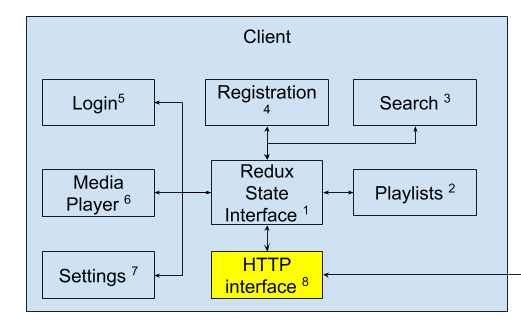
\includegraphics[width=0.60\textwidth]{images/client/client_http_interface.png}
 	\caption{Client-side HTTP interface subsystem}
\end{figure}


\subsubsection{Subsystem Operating System}
We need the Fetch API from Mozilla and will be using Chrome 42 or Firefox 39

\subsubsection{Subsystem Software Dependencies}
We will be using React.js 16.8.0-alpha.1 for our framework and will be using the Fetch API from Mozilla.

\subsubsection{Subsystem Programming Languages}
A description of any programming languages used is JavaScript ES6

\subsubsection{Subsystem Data Structures}
The first data structure is the a resource request with fetch(url-from-server)
The second data structure is the Response from the server which will be a JSON (key-pair values) object with the authorization, music,and specific playlists requested



\newpage